\documentclass[10pt,a4paper]{report}
\usepackage[latin1]{inputenc}
\usepackage{amsmath}
\usepackage{amsfonts}
\usepackage{amssymb}
\usepackage{graphicx}
\usepackage{hyperref}
\usepackage{multicol}
\usepackage[margin=0.5in]{geometry}
\usepackage{tikz}
\usepackage{romannum}
\usetikzlibrary{arrows,shapes.gates.logic.US,shapes.gates.logic.IEC,calc}
\usepackage{titlesec}
\titlespacing{\subsection}{1pt}{\parskip}{3pt}
\titlespacing{\subsubsection}{0pt}{\parskip}{-\parskip}
\titlespacing{\paragraph}{0pt}{\parskip}{\parskip}
\newcommand{\myvec}[1]{\ensuremath{\begin{pmatrix}#1\end{pmatrix}}}


\begin{document}

\centering {
\includegraphics[scale=0.07]{IITH.png}} \vspace{3mm}\\ \raggedleft Name:T.Manasa Reddy\vspace{2mm}\\ \raggedleft Roll No.: FWC22048\vspace{2mm}\\ \raggedright Sep 2022 \hspace{12cm} \raggedleft manasatanuboddi@gmail.com \vspace{10mm}
\\ \centering \Large \textbf{MATRIX ASSIGNMENT} \normalsize \vspace{15mm}

\begin{multicols}{2}

\section{Problem:}  Construct a triangle ABC in which BC=7cm, $\angle{B}=75^0$ and AB + AC = 13 cm \vspace{3mm}
 \section{Solution: }
\raggedright \textbf{Theory:}\\
\centering Construct a triangle ABC in which BC = 7cm, $\angle{B}=75^0$ and AB + AC = 13 \\

\raggedright \textbf{To Prove:}\\
i) Draw base BC = 7cm, and at point, B make an angle CBX of $\angle{B}=75^0$ using \centering a protractor. \\ 
ii) With B as center and radius BD = 13 cm, draw an arc to intersect ray BX at D. \\
iii) \raggedright Join DC. \\
iv) Let's construct a perpendicular bisector of DC. With D and C as the center \centering and radius greater than half of DC, draw arcs above and below the line DC to intersect ray BX at A. \\
v) \raggedright Join AC. 

\centering ABC is the required triangle. 

\raggedright\textbf{Verification:} 

On measuring we see that,BC = 7cm, $\angle{B}=75^0$ and  AB + AC = 13cm  \\
   \section{TermuxCommands: } 
               \centering python3 matrix.py

\raggedright \textbf{To Prove:}\\
   Given BC length is a=7cm,so the coordinates of B are 
 $\begin{pmatrix}
  0\\
  0 \\
 \end{pmatrix}$% 
 \\ X1,Y1 respectively and the cordinates of C are,
 $\begin{pmatrix}
  a\\
  0 \\
 \end{pmatrix}$%   
 \\ X3,Y3 respectively and also given the angle is $B=75^0$,so \\ by finding the coordinates of the other side we can form a required triangle. \\

\raggedright \textbf{Caluclating Other Coordinate: } \\
        \centering Let the coordinates of A are X2,Y2 respectively. \\
   Let A = $\begin{pmatrix} 
  sin \theta\\
  cos \theta\\
 \end{pmatrix}$% 
   Using the Cosine formula in  $\Delta$ABC, \\
    ${b}^2$ = ${a}^2$ + ${c}^2$ - 2accosB.\\
  \centering $\implies$ (b+c)(b-c)+${7}^2$ - 2 $\times$ 7 $\times$ 0.9217c \\
  \centering $\implies$ b-1.99c=3.76 ....1\\
   Upon Simplifaction we get:- \\
       b+c=$7$ ....2  \\
     and the above 2 equations can be written as:- \\
        $\begin{pmatrix}
            1 & -1.99  \\
            1 & -1  \\
        \end{pmatrix}$% 
        $\begin{pmatrix}
            b \\
            c \\
        \end{pmatrix}$% 
           =
           $\begin{pmatrix}
            3.76 \\
            13\\
        \end{pmatrix}$%              
   \\ from this, 
      $\begin{pmatrix}
            b\\
            c\\
        \end{pmatrix}$% 
            =
            $\begin{pmatrix}
            9.91\\
            -0.38\\
        \end{pmatrix}$% 
   \\  Thus,the vertices of $\Delta$ ABC are \\
     A= 9.91 $\begin{pmatrix}
                 cos 75\\
                 sin 75\\
              \end{pmatrix}$% 
              ,B= $\begin{pmatrix}
                 0\\
                 0\\
              \end{pmatrix}$% 
             ,C= $\begin{pmatrix}
                  7\\
                  0\\
              \end{pmatrix}$% 
              
The below python code realizes the above construction:	

 https://github.com/manasareddy442002/fwc-moudle1/blob/c70dd69787e4015345ac92e472d1d80a152f851d/matrix.py

        

 \section{Construction}
 	\begin{center}
  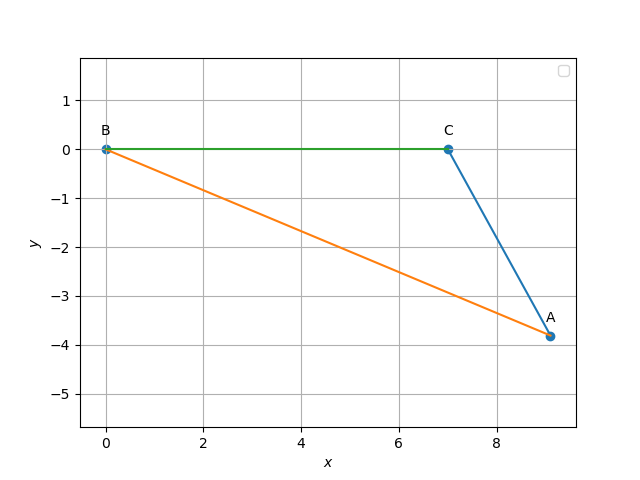
\includegraphics[scale=0.5]{Figure_1.png}
  	\end{center}
  


  



\vspace{3cm}


\end{multicols}

\end{document}
